\documentclass[12pt, a4paper]{article}

% Betöltjük a preamble.tex fájlt. Fontos a relatív elérési út!
\usepackage{booktabs}
\usepackage[T1]{fontenc}
\usepackage[utf8]{inputenc}
\usepackage[english]{babel}
\usepackage{amsmath, amssymb, amsthm} % Matek környezetek
\usepackage{geometry}
\geometry{
    a4paper,
    margin=2.5cm,
}
\usepackage{xcolor}
\usepackage{tikz}
\usepackage{float}
\usepackage{caption}
\usetikzlibrary{calc, positioning, arrows.meta, shapes.geometric, fit, matrix}

\tikzset{
    state/.style={
        matrix of nodes,
        nodes={
            draw=black!50, 
            minimum size=0.65cm, 
            anchor=center, 
            fill=white, 
            font=\ttfamily\footnotesize
        },
        column sep=-\pgflinewidth, 
        row sep=-\pgflinewidth,
        draw=black, 
        thick,
        inner sep=0pt
    },
    process/.style={rectangle, draw=black, thick, fill=white, align=center, minimum width=3.5cm, minimum height=0.8cm},
    block/.style={rectangle, draw=blue!80!black, thick, fill=blue!5, minimum width=2cm, minimum height=1cm, align=center, font=\bfseries},
    enc/.style={trapezium, trapezium angle=70, draw=black, thick, fill=gray!10, minimum width=2cm, align=center, shape border rotate=270},
    xor/.style={circle, draw=black, thick, inner sep=0pt, minimum size=0.4cm, path picture={\draw[thick] (path picture bounding box.north) -- (path picture bounding box.south) (path picture bounding box.west) -- (path picture bounding box.east);}},
    group/.style={rectangle, draw=gray, dashed, inner sep=0.3cm},
    arrow/.style={-Latex, thick},
    label/.style={font=\small\bfseries, color=gray!80!black, align=center},
    rsaStep/.style={rectangle, draw=black, thick, fill=white, align=center, minimum width=4cm, minimum height=0.8cm, rounded corners},
    data/.style={rectangle, draw=blue!80!black, thick, fill=blue!5, align=center, minimum width=2.5cm},
    arrow/.style={-Latex, thick},
    actor/.style={circle, draw=black, thick, minimum size=1.5cm, fill=gray!10, font=\bfseries},
    box/.style={rectangle, draw=black, thick, fill=white, align=center, minimum width=2.5cm, minimum height=1.5cm},
    op/.style={rectangle, draw=black, thick, fill=white, align=center, minimum width=3cm},
    decision/.style={diamond, draw=orange!80!black, thick, fill=orange!5, aspect=2, align=center, font=\small, inner sep=1pt},
    term/.style={rectangle, draw=black, thick, fill=gray!20, rounded corners, minimum height=0.8cm},
    elgamalStep/.style={rectangle, draw=black, thick, fill=white, align=center, minimum width=4cm, minimum height=0.8cm, rounded corners},
    secret/.style={rectangle, draw=red!80!black, thick, fill=red!10, align=center},
    public/.style={rectangle, draw=green!60!black, thick, fill=green!10, align=center},
    random/.style={diamond, draw=orange!80!black, thick, fill=orange!10, aspect=2, inner sep=2pt, font=\small, align=center},
    sigStep/.style={rectangle, draw=black, thick, fill=white, align=center, minimum width=4cm, minimum height=0.8cm, rounded corners},
    check/.style={diamond, draw=orange!80!black, thick, fill=orange!10, aspect=2, inner sep=2pt, font=\small, align=center},
    hash/.style={trapezium, draw=purple!80!black, thick, fill=purple!10, shape border rotate=270, align=center, minimum width=2cm}
}

\definecolor{kiemelt}{HTML}{0078A8}
\newcommand{\kiemeles}[1]{\textcolor{kiemelt}{\textbf{#1}}}

% Tételstílusok
\newtheoremstyle{tetelstilus}
    {\topsep}
    {\topsep}
    {\itshape}
    {}
    {\bfseries}
    {.}
    {.5em}
    {\thmname{#1}\thmnumber{ #2}\thmnote{ (\textbf{#3})}}
\theoremstyle{tetelstilus}

\newtheorem{defin}{Definíció}
\newtheorem{tetel}{Tétel}

\title{\LARGE\textbf{Machine Learning Basics}}




\begin{document}
\maketitle
\thispagestyle{empty} % A főcím oldalán eltávolítja az oldalszámot



% Global TikZ Styles
\tikzset{
    vector/.style={-Latex, very thick, blue},
    result/.style={-Latex, very thick, red},
    axis/.style={-Latex, thick, black},
    grid/.style={gray!30, very thin},
    matrixbox/.style={rectangle, draw=black, thick, fill=white, align=center, minimum width=1cm, minimum height=1cm}
}

\title{\textbf{Linear Algebra: Concepts \& Examples}}
\author{Comprehensive Guide}
\date{}


\maketitle
\tableofcontents
\newpage

\section{Vectors}
A vector is an ordered list of numbers, geometrically representing a magnitude and direction.

\subsection{Definition and Operations}
Let $\mathbf{u}, \mathbf{v} \in \mathbb{R}^n$.
\begin{itemize}
    \item \textbf{Column Vector:} $\mathbf{u} = \begin{bmatrix} u_1 \\ u_2 \\ \vdots \\ u_n \end{bmatrix}$.
    \item \textbf{Addition:} $\mathbf{u} + \mathbf{v}$ adds components element-wise.
    \item \textbf{Dot Product:} $\mathbf{u} \cdot \mathbf{v} = \sum u_i v_i$.
    \item \textbf{Norm (Length):} $\|\mathbf{u}\| = \sqrt{\mathbf{u} \cdot \mathbf{u}}$.
\end{itemize}

\subsection{Example}
Let $\mathbf{u} = \begin{bmatrix} 2 \\ 1 \end{bmatrix}$ and $\mathbf{v} = \begin{bmatrix} 1 \\ 3 \end{bmatrix}$.
\begin{align*}
    \mathbf{u} + \mathbf{v} &= \begin{bmatrix} 2+1 \\ 1+3 \end{bmatrix} = \begin{bmatrix} 3 \\ 4 \end{bmatrix} \\
    \mathbf{u} \cdot \mathbf{v} &= (2)(1) + (1)(3) = 5 \\
    \|\mathbf{u}\| &= \sqrt{2^2 + 1^2} = \sqrt{5} \approx 2.236
\end{align*}

\begin{figure}[H]
    \centering
    \begin{tikzpicture}[scale=1.2]
        \draw[grid] (-1,-1) grid (4,5);
        \draw[axis] (-1,0) -- (4.2,0) node[right] {$x$};
        \draw[axis] (0,-1) -- (0,5.2) node[above] {$y$};
        
        \draw[vector] (0,0) -- (2,1) node[midway, below right] {$\mathbf{u}$};
        \draw[vector] (0,0) -- (1,3) node[midway, left] {$\mathbf{v}$};
        
        \draw[dashed, gray] (2,1) -- (3,4);
        \draw[dashed, gray] (1,3) -- (3,4);
        \draw[result] (0,0) -- (3,4) node[above right] {$\mathbf{u}+\mathbf{v}$};
    \end{tikzpicture}
    \caption{Vector Addition (Parallelogram Rule).}
\end{figure}

\section{Matrices}
A matrix is a rectangular array of numbers. An $m \times n$ matrix has $m$ rows and $n$ columns.

\subsection{Matrix Multiplication}
If $A$ is $m \times n$ and $B$ is $n \times p$, then $C = AB$ is $m \times p$.
\[ c_{ij} = \text{Row}_i(A) \cdot \text{Col}_j(B) \]

\subsection{Example}
Let $A = \begin{bmatrix} 1 & 2 \\ 3 & 4 \end{bmatrix}$ and $B = \begin{bmatrix} 2 & 0 \\ 1 & 2 \end{bmatrix}$.
\[
AB = \begin{bmatrix} (1)(2) + (2)(1) & (1)(0) + (2)(2) \\ (3)(2) + (4)(1) & (3)(0) + (4)(2) \end{bmatrix} 
= \begin{bmatrix} 4 & 4 \\ 10 & 8 \end{bmatrix}
\]

\section{3. Determinants}
The determinant is a scalar value associated with a square matrix that encodes scaling properties (like area or volume). If $\det(A) = 0$, the matrix is singular (not invertible).

\subsection{Definitions}
\begin{itemize}
    \item \textbf{2x2 Matrix:} $\det \begin{bmatrix} a & b \\ c & d \end{bmatrix} = ad - bc$.
    \item \textbf{3x3 Matrix:} Uses cofactor expansion (e.g., across top row).
\end{itemize}

\subsection{Example}
Let $A = \begin{bmatrix} 2 & 5 \\ 1 & 3 \end{bmatrix}$.
\[
\det(A) = (2)(3) - (5)(1) = 6 - 5 = 1
\]
Since $\det(A) \neq 0$, $A$ is invertible.

\section{4. Matrix Inversion}
The inverse $A^{-1}$ of a square matrix $A$ satisfies $AA^{-1} = A^{-1}A = I$ (Identity Matrix).

\subsection{Formula (2x2)}
\[
A^{-1} = \frac{1}{\det(A)} \begin{bmatrix} d & -b \\ -c & a \end{bmatrix}
\]

\subsection{Example}
Using $A$ from the section above ($\det(A)=1$):
\[
A^{-1} = \frac{1}{1} \begin{bmatrix} 3 & -5 \\ -1 & 2 \end{bmatrix} = \begin{bmatrix} 3 & -5 \\ -1 & 2 \end{bmatrix}
\]
\textbf{Check:}
\[
AA^{-1} = \begin{bmatrix} 2 & 5 \\ 1 & 3 \end{bmatrix} \begin{bmatrix} 3 & -5 \\ -1 & 2 \end{bmatrix} = \begin{bmatrix} 6-5 & -10+10 \\ 3-3 & -5+6 \end{bmatrix} = \begin{bmatrix} 1 & 0 \\ 0 & 1 \end{bmatrix}
\]

\section{Gaussian Elimination}
An algorithm to solve systems of linear equations of the form $A\mathbf{x} = \mathbf{b}$.
We form the \textbf{Augmented Matrix} $[A | \mathbf{b}]$ and perform row operations to reach \textbf{Row Echelon Form (REF)}.

\subsection{Example System}
\[
\begin{cases}
x + 2y + z = 8 \\
2x + 5y + 3z = 19 \\
-x + y + 2z = 5
\end{cases}
\implies
\left[ \begin{array}{ccc|c} 
1 & 2 & 1 & 8 \\ 
2 & 5 & 3 & 19 \\ 
-1 & 1 & 2 & 5 
\end{array} \right]
\]

\textbf{Step 1:} Eliminate $x$ from rows 2 and 3.
\begin{itemize}
    \item $R_2 \leftarrow R_2 - 2R_1$
    \item $R_3 \leftarrow R_3 + R_1$
\end{itemize}
\[
\left[ \begin{array}{ccc|c} 
1 & 2 & 1 & 8 \\ 
0 & 1 & 1 & 3 \\ 
0 & 3 & 3 & 13 
\end{array} \right]
\]

\textbf{Step 2:} Eliminate $y$ from row 3.
\begin{itemize}
    \item $R_3 \leftarrow R_3 - 3R_2$
\end{itemize}
\[
\left[ \begin{array}{ccc|c} 
1 & 2 & 1 & 8 \\ 
0 & 1 & 1 & 3 \\ 
0 & 0 & 0 & 4 
\end{array} \right]
\]
\textbf{Analysis:} The last row says $0x + 0y + 0z = 4$, which is impossible ($0 \neq 4$).
\textbf{Conclusion:} This system has \textbf{No Solution} (Inconsistent).

\section{6. Eigenvalues and Eigenvectors}
An eigenvector of a square matrix $A$ is a non-zero vector $\mathbf{v}$ such that $A\mathbf{v} = \lambda \mathbf{v}$, where $\lambda$ is a scalar (eigenvalue).

\subsection{Algorithm}
\begin{enumerate}
    \item Solve the characteristic equation $\det(A - \lambda I) = 0$ to find $\lambda$.
    \item For each $\lambda$, solve $(A - \lambda I)\mathbf{v} = \mathbf{0}$ to find $\mathbf{v}$.
\end{enumerate}

\subsection{Example}
Let $A = \begin{bmatrix} 4 & 1 \\ 2 & 3 \end{bmatrix}$.

\textbf{1. Find Eigenvalues:}
\[
\det \left( \begin{bmatrix} 4 & 1 \\ 2 & 3 \end{bmatrix} - \lambda \begin{bmatrix} 1 & 0 \\ 0 & 1 \end{bmatrix} \right) = \det \begin{bmatrix} 4-\lambda & 1 \\ 2 & 3-\lambda \end{bmatrix}
\]
\[
(4-\lambda)(3-\lambda) - 2 = \lambda^2 - 7\lambda + 12 - 2 = \lambda^2 - 7\lambda + 10 = 0
\]
Factoring $(\lambda - 5)(\lambda - 2) = 0$ gives eigenvalues $\lambda_1 = 5, \lambda_2 = 2$.

\textbf{2. Find Eigenvector for $\lambda_1 = 5$:}
Solve $(A - 5I)\mathbf{v} = \mathbf{0}$:
\[
\begin{bmatrix} 4-5 & 1 \\ 2 & 3-5 \end{bmatrix} \begin{bmatrix} x \\ y \end{bmatrix} = \begin{bmatrix} -1 & 1 \\ 2 & -2 \end{bmatrix} \begin{bmatrix} x \\ y \end{bmatrix} = \begin{bmatrix} 0 \\ 0 \end{bmatrix}
\]
$-x + y = 0 \implies x = y$. Let $x=1$, then $y=1$.
Eigenvector $\mathbf{v}_1 = \begin{bmatrix} 1 \\ 1 \end{bmatrix}$.

\begin{figure}[H]
    \centering
    \begin{tikzpicture}[scale=0.8]
        \draw[grid] (-1,-1) grid (6,6);
        \draw[axis] (-1,0) -- (6,0) node[right] {$x$};
        \draw[axis] (0,-1) -- (0,6) node[above] {$y$};
        
        % Original vector
        \draw[vector] (0,0) -- (1,1) node[midway, left] {$\mathbf{v}$};
        
        % Transformed vector
        \draw[result] (0,0) -- (5,5) node[right] {$A\mathbf{v} = 5\mathbf{v}$};
        
        \node[align=left, fill=white] at (2, 4) {Direction is preserved.\\Scaled by $\lambda=5$.};
    \end{tikzpicture}
    \caption{Visualizing the Eigenvector transformation.}
\end{figure}


\section{Random Variables and Distributions}
A \textbf{Random Variable} (RV) is a function that maps outcomes of a random experiment to real numbers. It translates experimental outcomes into numerical data.

\subsection{Discrete vs. Continuous}
\begin{itemize}
    \item \textbf{Discrete Random Variable:} Can only take on a countable number of distinct values (e.g., outcome of a dice roll, number of heads in 10 tosses).
    \item \textbf{Continuous Random Variable:} Can take on any value within an interval (e.g., height, temperature, time).
\end{itemize}

\subsection{Probability Functions}
\begin{itemize}
    \item \textbf{Discrete:} Described by a \textbf{Probability Mass Function (PMF)}, denoted $P(X=x)$.
    \item \textbf{Continuous:} Described by a \textbf{Probability Density Function (PDF)}, denoted $f(x)$. Probabilities are areas under the curve:
    \[ P(a \le X \le b) = \int_{a}^{b} f(x) \, dx \]
    \textit{Note: For continuous variables, the probability of any single exact point is zero ($P(X=c) = 0$).}
\end{itemize}

\subsection{Expected Value (Mean)}
The expected value $E[X]$ (often denoted $\mu$) is the theoretical long-run average of the random variable. It is a measure of the "center" of the distribution.

\begin{itemize}
    \item \textbf{Discrete Case:} Weighted sum of values.
    \[ E[X] = \sum_{i} x_i \cdot P(X = x_i) \]
    \textit{Example (Fair Die):} $E[X] = 1(\frac{1}{6}) + \dots + 6(\frac{1}{6}) = 3.5$.
    
    \item \textbf{Continuous Case:} Integral of value weighted by density.
    \[ E[X] = \int_{-\infty}^{\infty} x \cdot f(x) \, dx \]
\end{itemize}

\section{Common Distributions}

\subsection{Uniform Distribution}
In a uniform distribution, all outcomes in the sample space are equally likely.

\textbf{1. Discrete Uniform ($U\{a, b\}$):}
A finite set of values $\{a, a+1, \dots, b\}$ where each outcome has probability $\frac{1}{n}$.
\[ E[X] = \frac{a+b}{2} \]

\textbf{2. Continuous Uniform ($U[a, b]$):}
The probability density is constant over the interval $[a, b]$.
\[ f(x) = \begin{cases} \frac{1}{b-a} & \text{if } a \le x \le b \\ 0 & \text{otherwise} \end{cases} \]
\[ E[X] = \frac{a+b}{2} \]

\begin{figure}[H]
    \centering
    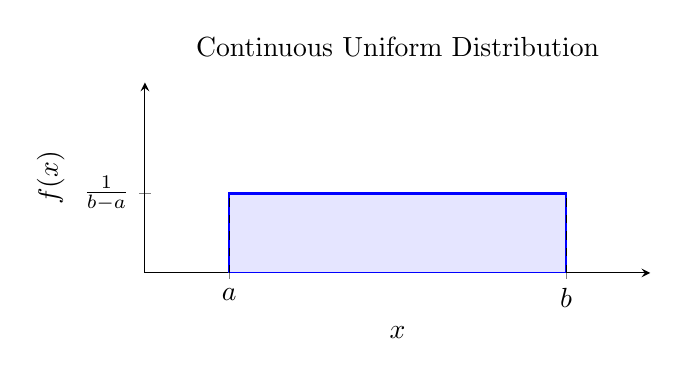
\begin{tikzpicture}
        \begin{axis}[
            width=8cm, height=4cm,
            axis lines=left,
            xlabel=$x$, ylabel=$f(x)$,
            ymin=0, ymax=0.6,
            xmin=0, xmax=6,
            xtick={1, 5}, xticklabels={$a$, $b$},
            ytick={0.25}, yticklabels={$\frac{1}{b-a}$},
            title={Continuous Uniform Distribution}
        ]
            \addplot[blue, thick, fill=blue!10] coordinates {(1,0.25) (5,0.25)} \closedcycle;
            \addplot[dashed] coordinates {(1,0) (1,0.25)};
            \addplot[dashed] coordinates {(5,0) (5,0.25)};
        \end{axis}
    \end{tikzpicture}
    \caption{The PDF of a Continuous Uniform Distribution.}
\end{figure}

\subsection{Normal (Gaussian) Distribution}
The Normal distribution is the most important continuous distribution in statistics. It is symmetric, bell-shaped, and defined entirely by its mean ($\mu$) and variance ($\sigma^2$).
\[ X \sim \mathcal{N}(\mu, \sigma^2) \]

\textbf{PDF Formula:}
\[ f(x) = \frac{1}{\sigma\sqrt{2\pi}} e^{-\frac{1}{2}\left(\frac{x-\mu}{\sigma}\right)^2} \]

\begin{figure}[H]
    \centering
    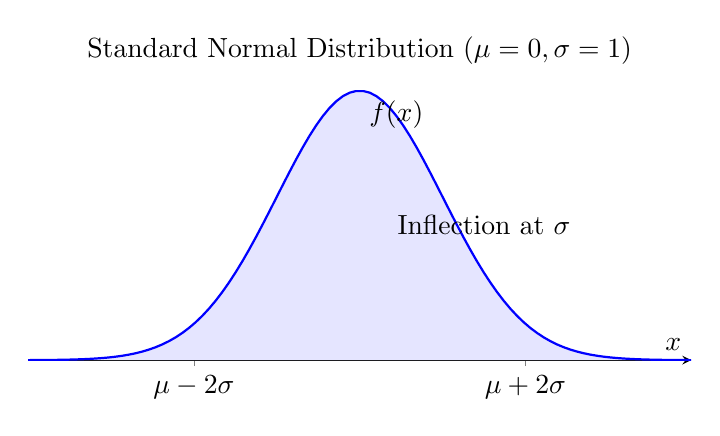
\begin{tikzpicture}
        \begin{axis}[
            width=10cm, height=5cm,
            axis lines=middle,
            domain=-4:4, samples=100,
            xlabel=$x$, ylabel=$f(x)$,
            xtick={-2, 0, 2}, xticklabels={$\mu-2\sigma$, $\mu$, $\mu+2\sigma$},
            ytick=\empty,
            title={Standard Normal Distribution ($\mu=0, \sigma=1$)}
        ]
            \addplot [thick, blue, fill=blue!10] {1/sqrt(2*pi)*exp(-x^2/2)};
            \node[anchor=south] at (axis cs: 0, 0.4) {Peak at $\mu$};
            \node at (axis cs: 1.5, 0.2) {Inflection at $\sigma$};
        \end{axis}
    \end{tikzpicture}
    \caption{The Normal Distribution (Bell Curve). 68\% of data falls within $\mu \pm \sigma$.}
\end{figure}

\section{Normal Equation (Normál Egyenlet)}
For Linear Regression, the minimum of the cost function can be found analytically in a closed form without iteration. By setting the gradient to zero, we get:
\[
\theta = (X^T X)^{-1} X^T \mathbf{y}
\]
\begin{itemize}
    \item \textbf{Pros:} No need to choose a learning rate; gives an exact solution immediately.
    \item \textbf{Cons:} Computationally expensive for large datasets because inverting the matrix $(X^T X)$ has a complexity of $O(n^3)$ (where $n$ is the number of features).
\end{itemize}

\subsection*{Example Calculation}
Suppose we have a tiny dataset with 3 points: $(1, 1), (2, 2), (3, 2)$. We want to fit a line $y = \theta_0 + \theta_1 x$.

\textbf{1. Construct Matrices:}
Add a column of 1s for the bias term $\theta_0$.
\[
X = \begin{bmatrix} 1 & 1 \\ 1 & 2 \\ 1 & 3 \end{bmatrix}, \quad
\mathbf{y} = \begin{bmatrix} 1 \\ 2 \\ 2 \end{bmatrix}
\]

\textbf{2. Compute $X^T X$:}
\[
X^T X = \begin{bmatrix} 1 & 1 & 1 \\ 1 & 2 & 3 \end{bmatrix} 
\begin{bmatrix} 1 & 1 \\ 1 & 2 \\ 1 & 3 \end{bmatrix} 
= \begin{bmatrix} 3 & 6 \\ 6 & 14 \end{bmatrix}
\]

\textbf{3. Compute Inverse $(X^T X)^{-1}$:}
Using the formula for 2x2 inverse:
\[
\text{det} = 3(14) - 6(6) = 42 - 36 = 6
\]
\[
(X^T X)^{-1} = \frac{1}{6} \begin{bmatrix} 14 & -6 \\ -6 & 3 \end{bmatrix}
\]

\textbf{4. Compute $X^T \mathbf{y}$:}
\[
X^T \mathbf{y} = \begin{bmatrix} 1 & 1 & 1 \\ 1 & 2 & 3 \end{bmatrix} 
\begin{bmatrix} 1 \\ 2 \\ 2 \end{bmatrix}
= \begin{bmatrix} 1+2+2 \\ 1+4+6 \end{bmatrix} 
= \begin{bmatrix} 5 \\ 11 \end{bmatrix}
\]

\textbf{5. Solve for $\theta$:}
\[
\theta = \frac{1}{6} \begin{bmatrix} 14 & -6 \\ -6 & 3 \end{bmatrix} 
\begin{bmatrix} 5 \\ 11 \end{bmatrix} 
= \frac{1}{6} \begin{bmatrix} 70 - 66 \\ -30 + 33 \end{bmatrix} 
= \frac{1}{6} \begin{bmatrix} 4 \\ 3 \end{bmatrix} 
= \begin{bmatrix} 2/3 \\ 1/2 \end{bmatrix}
\]
Result: $\theta_0 \approx 0.67$ (Intercept), $\theta_1 = 0.5$ (Slope).



\section{1. Feature Normalization (Leírók Normalizálása)}
Machine learning algorithms (e.g., Gradient Descent, k-NN) often perform poorly if the input features have vastly different scales (e.g., Age [0-100] vs. Salary [1000-10000]). Normalization aims to bring features to a common scale.

\subsection{Standardization (Z-score Normalization)}
Data is transformed so that the mean ($\mu$) is 0 and the standard deviation ($\sigma$) is 1. This is the most common method (used in PCA, Logistic Regression, etc.).
\[
x' = \frac{x - \mu}{\sigma}
\]

\subsection{Min-Max Scaling}
Maps the data to a fixed interval, typically $[0, 1]$.
\[
x' = \frac{x - \min(x)}{\max(x) - \min(x)}
\]
\textit{Disadvantage:} It is highly sensitive to outliers.


\subsection{Normal Equation (Normál Egyenlet)}
For Linear Regression, the minimum of the cost function can be found analytically in a closed form without iteration. By setting the gradient to zero, we get:
\[
\theta = (X^T X)^{-1} X^T \mathbf{y}
\]
\begin{itemize}
    \item \textbf{Pros:} No need to choose a learning rate; gives an exact solution immediately.
    \item \textbf{Cons:} Computationally expensive for large datasets because inverting the matrix $(X^T X)$ has a complexity of $O(n^3)$ (where $n$ is the number of features).
\end{itemize}

\subsubsection*{Example Calculation}
Suppose we have a tiny dataset with 3 points: $(1, 1), (2, 2), (3, 2)$. We want to fit a line $y = \theta_0 + \theta_1 x$.

\textbf{1. Construct Matrices:}
Add a column of 1s for the bias term $\theta_0$.
\[
X = \begin{bmatrix} 1 & 1 \\ 1 & 2 \\ 1 & 3 \end{bmatrix}, \quad
\mathbf{y} = \begin{bmatrix} 1 \\ 2 \\ 2 \end{bmatrix}
\]

\textbf{2. Compute $X^T X$:}
\[
X^T X = \begin{bmatrix} 1 & 1 & 1 \\ 1 & 2 & 3 \end{bmatrix} 
\begin{bmatrix} 1 & 1 \\ 1 & 2 \\ 1 & 3 \end{bmatrix} 
= \begin{bmatrix} 3 & 6 \\ 6 & 14 \end{bmatrix}
\]

\textbf{3. Compute Inverse $(X^T X)^{-1}$:}
Using the formula for 2x2 inverse:
\[
\text{det} = 3(14) - 6(6) = 42 - 36 = 6
\]
\[
(X^T X)^{-1} = \frac{1}{6} \begin{bmatrix} 14 & -6 \\ -6 & 3 \end{bmatrix}
\]

\textbf{4. Compute $X^T \mathbf{y}$:}
\[
X^T \mathbf{y} = \begin{bmatrix} 1 & 1 & 1 \\ 1 & 2 & 3 \end{bmatrix} 
\begin{bmatrix} 1 \\ 2 \\ 2 \end{bmatrix}
= \begin{bmatrix} 1+2+2 \\ 1+4+6 \end{bmatrix} 
= \begin{bmatrix} 5 \\ 11 \end{bmatrix}
\]

\textbf{5. Solve for $\theta$:}
\[
\theta = \frac{1}{6} \begin{bmatrix} 14 & -6 \\ -6 & 3 \end{bmatrix} 
\begin{bmatrix} 5 \\ 11 \end{bmatrix} 
= \frac{1}{6} \begin{bmatrix} 70 - 66 \\ -30 + 33 \end{bmatrix} 
= \frac{1}{6} \begin{bmatrix} 4 \\ 3 \end{bmatrix} 
= \begin{bmatrix} 2/3 \\ 1/2 \end{bmatrix}
\]
Result: $\theta_0 \approx 0.67$ (Intercept), $\theta_1 = 0.5$ (Slope).

\section{Probability Theory}

\subsection{Univariate Normal Distribution (Egyváltozós Normális Eloszlás)}
The most common distribution in nature (Gaussian). Defined by mean $\mu$ and variance $\sigma^2$:
\[
p(x) = \frac{1}{\sqrt{2\pi\sigma^2}} \exp\left( -\frac{(x-\mu)^2}{2\sigma^2} \right)
\]

\begin{figure}[H]
    \centering
    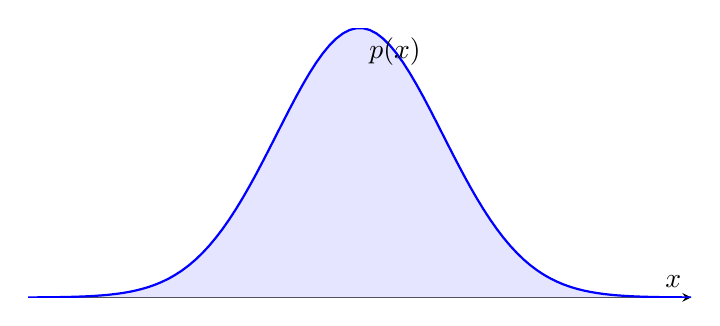
\begin{tikzpicture}
        \begin{axis}[
            domain=-4:4, samples=100,
            axis lines=middle,
            height=5cm, width=10cm,
            xlabel=$x$, ylabel=$p(x)$,
            xtick={0}, xticklabels={$\mu$},
            ytick=\empty
        ]
            \addplot [thick, blue, fill=blue!10] {exp(-x^2/2)};
        \end{axis}
    \end{tikzpicture}
    \caption{Standard Normal Distribution.}
\end{figure}

\subsection{Multivariate Normal Distribution (Többváltozós Normális Eloszlás)}
Generalization to $k$ dimensions. Defined by the mean vector $\boldsymbol{\mu}$ and the covariance matrix $\Sigma$:
\[
p(\mathbf{x}) = \frac{1}{\sqrt{(2\pi)^k |\Sigma|}} \exp\left( -\frac{1}{2} (\mathbf{x} - \boldsymbol{\mu})^T \Sigma^{-1} (\mathbf{x} - \boldsymbol{\mu}) \right)
\]
Important for algorithms like Gaussian Mixture Models (GMM) and Linear Discriminant Analysis (LDA).

\section{ Dimensionality Reduction}

\subsection{Principal Component Analysis (PCA)}
PCA reduces the dimensionality of the data while preserving as much variance (information) as possible.
\textbf{Steps:}
\begin{enumerate}
    \item \textbf{Standardize} the data.
    \item Compute the \textbf{Covariance Matrix} $\Sigma$.
    \item Compute the \textbf{Eigenvectors} and \textbf{Eigenvalues} of $\Sigma$.
    \item Keep the top $k$ eigenvectors corresponding to the largest eigenvalues (Principal Components).
    \item Project the original data onto these components.
\end{enumerate}

\begin{figure}[H]
    \centering
    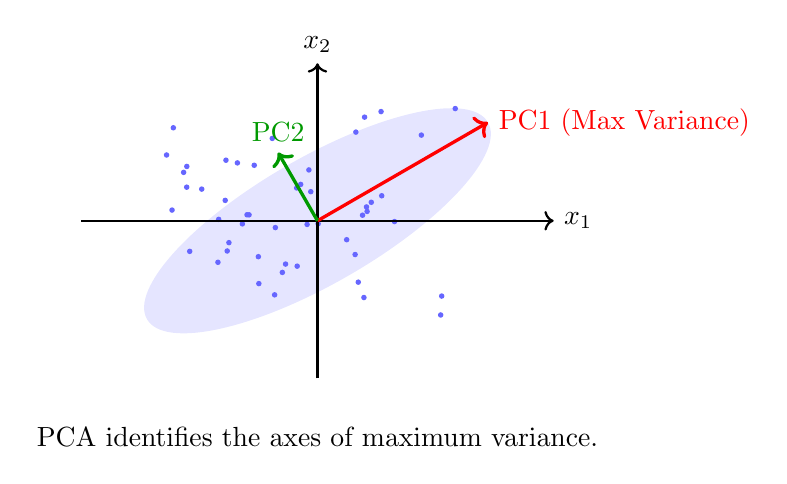
\begin{tikzpicture}
        % Data Cloud
        \draw[rotate=30, fill=blue!10, draw=none] (0,0) ellipse (2.5cm and 0.8cm);
        \foreach \i in {1,...,50} {
            \fill[blue!60] ({2*rand*cos(30) - 0.6*rand*sin(30)}, {2*rand*sin(30) + 0.6*rand*cos(30)}) circle (1pt);
        }
        
        % Axes
        \draw[->, thick] (-3,0) -- (3,0) node[right] {$x_1$};
        \draw[->, thick] (0,-2) -- (0,2) node[above] {$x_2$};
        
        % PC vectors
        \draw[->, very thick, red] (0,0) -- (30:2.5) node[right] {PC1 (Max Variance)};
        \draw[->, very thick, green!60!black] (0,0) -- (120:1) node[above] {PC2};
        
        \node[align=center, below=2.5cm] {PCA identifies the axes of maximum variance.};
    \end{tikzpicture}
    \caption{Concept of PCA: Finding the intrinsic axes of the data.}
\end{figure}

\section{Dimensionality Reduction}

\subsection{Principal Component Analysis (PCA)}
Principal Component Analysis (PCA) is an unsupervised learning algorithm used for dimensionality reduction. It identifies the "principal components"—linear combinations of the original features—that capture the maximum variance in the data.

\subsubsection{Geometric Intuition}
Imagine a cloud of data points in 2D. PCA finds a new coordinate system such that:
\begin{enumerate}
    \item The first axis (Principal Component 1 or PC1) aligns with the direction of greatest spread (variance) in the data.
    \item The second axis (PC2) is orthogonal (perpendicular) to the first and captures the remaining variance.
\end{enumerate}
By projecting data onto just PC1, we reduce the data from 2D to 1D while losing the least amount of information.

\subsubsection{The Algorithm Steps}
\begin{enumerate}
    \item \textbf{Data Preprocessing:}
    Standardize the data (as described in Section 1) so that each feature has mean 0 and variance 1. Let this matrix be $X$ (size $m \times n$).

    \item \textbf{Compute Covariance Matrix:}
    The covariance matrix $\Sigma$ expresses how features vary together.
    \[
    \Sigma = \frac{1}{m} X^T X
    \]
    $\Sigma$ is an $n \times n$ symmetric matrix.

    \item \textbf{Eigenvalue Decomposition:}
    Compute the eigenvectors and eigenvalues of $\Sigma$.
    \[
    \Sigma U = \lambda U
    \]
    \begin{itemize}
        \item \textbf{Eigenvectors ($U$):} Unit vectors representing the direction of the new axes.
        \item \textbf{Eigenvalues ($\lambda$):} Scalars representing the amount of variance captured by each eigenvector.
    \end{itemize}
    In practice, we often use Singular Value Decomposition (SVD) on $X$ for numerical stability.

    \item \textbf{Select Principal Components:}
    Sort eigenvectors by descending eigenvalues. Choose the top $k$ eigenvectors to form a transformation matrix $U_{reduce}$ ($n \times k$).

    \item \textbf{Project Data:}
    Transform the original data $X$ into the new lower-dimensional subspace $Z$.
    \[
    Z = X \cdot U_{reduce}
    \]
    The resulting $Z$ is size $m \times k$.
\end{enumerate}

\subsubsection{Choosing $k$ (Explained Variance)}
How many components should we keep? We look at the \textit{Explained Variance Ratio}. The variance explained by the $i$-th component is proportional to its eigenvalue $\lambda_i$.
\[
\frac{\sum_{i=1}^k \lambda_i}{\sum_{j=1}^n \lambda_j} \ge 0.95 \quad (\text{e.g., 95\% variance retained})
\]

\begin{figure}[H]
    \centering
    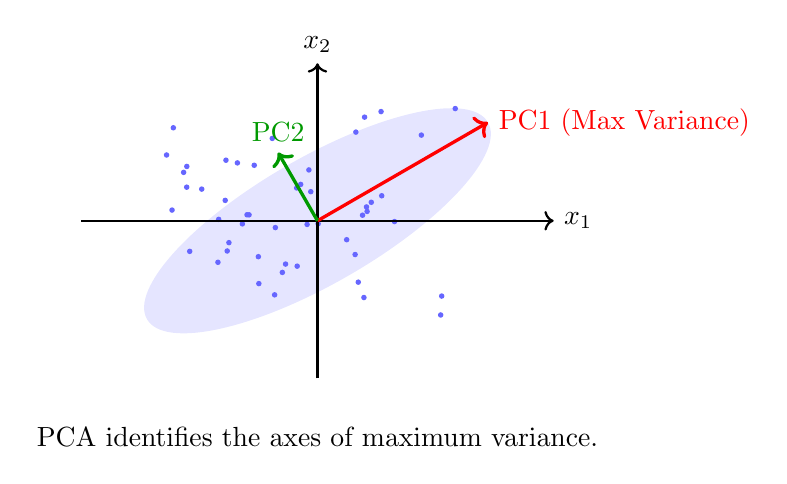
\begin{tikzpicture}
        % Data Cloud
        \draw[rotate=30, fill=blue!10, draw=none] (0,0) ellipse (2.5cm and 0.8cm);
        \foreach \i in {1,...,50} {
            \fill[blue!60] ({2*rand*cos(30) - 0.6*rand*sin(30)}, {2*rand*sin(30) + 0.6*rand*cos(30)}) circle (1pt);
        }
        
        % Axes
        \draw[->, thick] (-3,0) -- (3,0) node[right] {$x_1$};
        \draw[->, thick] (0,-2) -- (0,2) node[above] {$x_2$};
        
        % PC vectors
        \draw[->, very thick, red] (0,0) -- (30:2.5) node[right] {PC1 (Max Variance)};
        \draw[->, very thick, green!60!black] (0,0) -- (120:1) node[above] {PC2};
        
        \node[align=center, below=2.5cm] {PCA identifies the axes of maximum variance.};
    \end{tikzpicture}
    \caption{Concept of PCA: Finding the intrinsic axes of the data.}
\end{figure}

\section{Regression Analysis (Regresszió)}

\subsection{Linear Regression (Lineáris Regresszió)}
Linear regression attempts to model the relationship between variables by fitting a linear equation to observed data.

\subsubsection{Univariate (Egyváltozós)}
Predicting a target $y$ based on a single feature $x$.
\[ h_\theta(x) = \theta_0 + \theta_1 x \]

\subsubsection{Multivariate (Többváltozós)}
Predicting $y$ based on multiple features $x_1, x_2, \dots, x_n$. We define $x_0 = 1$ (bias term).
\[ h_\theta(\mathbf{x}) = \theta_0 x_0 + \theta_1 x_1 + \dots + \theta_n x_n = \boldsymbol{\theta}^T \mathbf{x} \]

\subsubsection{Cost Function: Mean Squared Error (MSE)}
The objective is to minimize the average squared difference between predictions and actual values:
\[ J(\boldsymbol{\theta}) = \frac{1}{2m} \sum_{i=1}^m (h_\theta(\mathbf{x}^{(i)}) - y^{(i)})^2 \]

\subsection{Polynomial Regression (Polinomiális Regresszió)}
Used when data is non-linear. We create new features by raising original features to powers (e.g., $x^2, x^3$).
\[ h_\theta(x) = \theta_0 + \theta_1 x + \theta_2 x^2 + \dots + \theta_d x^d \]
Although the curve is non-linear, the problem remains \textit{linear in the parameters} $\theta$, so the normal equation or gradient descent can still be used.

\subsection{Logistic Regression (Logisztikus Regresszió)}
Despite the name, this is a **classification** algorithm for predicting probabilities (values between 0 and 1). It uses the **Sigmoid (Logistic) Function**:
\[ g(z) = \frac{1}{1 + e^{-z}} \]
The hypothesis becomes:
\[ h_\theta(\mathbf{x}) = g(\boldsymbol{\theta}^T \mathbf{x}) = \frac{1}{1 + e^{-\boldsymbol{\theta}^T \mathbf{x}}} \]
This represents the probability that the output is 1: $P(y=1 | \mathbf{x}; \boldsymbol{\theta})$.

\begin{figure}[H]
    \centering
    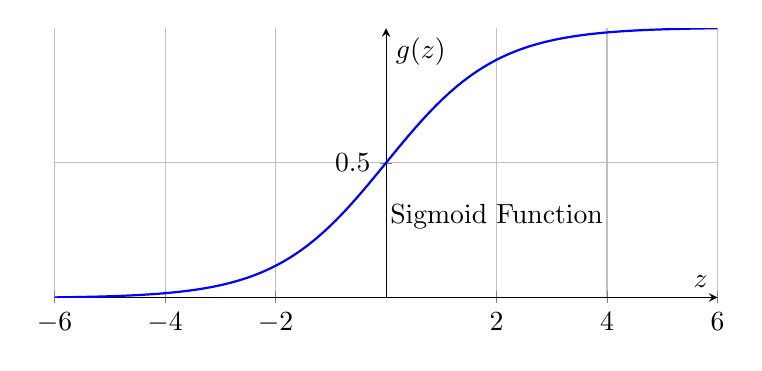
\begin{tikzpicture}
        \begin{axis}[
            domain=-6:6, samples=100,
            axis lines=middle,
            xlabel=$z$, ylabel=$g(z)$,
            height=5cm, width=10cm,
            ytick={0, 0.5, 1},
            grid=major
        ]
            \addplot [thick, blue] {1/(1+exp(-x))};
            \node at (axis cs:2, 0.3) {Sigmoid Function};
        \end{axis}
    \end{tikzpicture}
    \caption{The Sigmoid function maps any real number to the $(0, 1)$ interval.}
\end{figure}

\subsubsection{Cost Function: Binary Cross-Entropy (Log Loss)}
We cannot use MSE for Logistic Regression because the Sigmoid function makes the cost non-convex (multiple local minima). Instead, we use the Log Loss:
\[
\text{Cost}(h_\theta(\mathbf{x}), y) = 
\begin{cases} 
-\log(h_\theta(\mathbf{x})) & \text{if } y = 1 \\
-\log(1 - h_\theta(\mathbf{x})) & \text{if } y = 0 
\end{cases}
\]
Combined into a single equation:
\[ J(\boldsymbol{\theta}) = - \frac{1}{m} \sum_{i=1}^m \left[ y^{(i)} \log(h_\theta(\mathbf{x}^{(i)})) + (1 - y^{(i)}) \log(1 - h_\theta(\mathbf{x}^{(i)})) \right] \]

\begin{figure}[H]
    \centering
    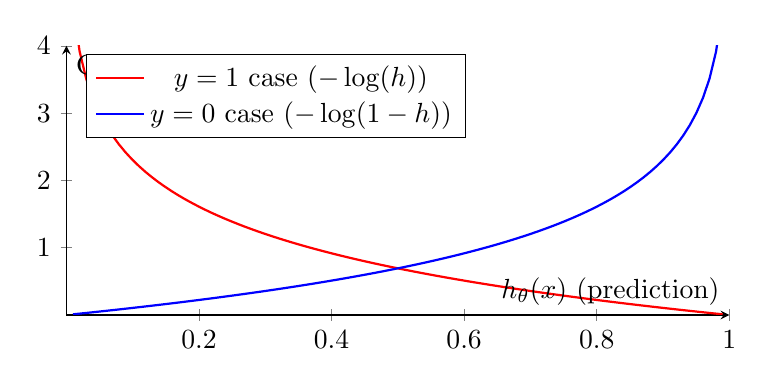
\begin{tikzpicture}
        \begin{axis}[
            domain=0.01:0.99, samples=100,
            axis lines=middle,
            xlabel=$h_\theta(x)$ (prediction), ylabel=Cost,
            height=5cm, width=10cm,
            xmin=0, xmax=1, ymin=0, ymax=4,
            legend pos=north west
        ]
            \addplot [thick, red] {-ln(x)};
            \addlegendentry{$y=1$ case ($-\log(h)$)}
            
            \addplot [thick, blue] {-ln(1-x)};
            \addlegendentry{$y=0$ case ($-\log(1-h)$)}
        \end{axis}
    \end{tikzpicture}
    \caption{Log Loss penalties. If $y=1$ and prediction $\approx 0$, cost $\to \infty$.}
\end{figure}

\section{Classification (Osztályozás)}

\subsection{Binary Classification (Bináris Osztályozás)}
The target variable $y$ has only two possible values: $0$ (Negative Class) or $1$ (Positive Class). Logistic regression uses a threshold (usually 0.5) to decide the class:
\[ \text{Predict } y=1 \text{ if } h_\theta(\mathbf{x}) \ge 0.5 \implies \boldsymbol{\theta}^T \mathbf{x} \ge 0 \]

\subsection{Multi-class Classification (Többosztályos Osztályozás)}
When $y$ can take on $k > 2$ values (e.g., classifying digits 0-9).

\paragraph{One-vs-All (One-vs-Rest):} Train $k$ separate binary classifiers.
\begin{itemize}
    \item Classifier $i$: Distinguish class $i$ from all other classes.
    \item Prediction: Choose the class $i$ that maximizes $h_\theta^{(i)}(\mathbf{x})$.
\end{itemize}

\section{Regularization (Regularizáció)}

\subsection{Overfitting vs. Underfitting (Túlillesztés és Alulillesztés)}
\begin{itemize}
    \item \textbf{Underfitting (High Bias):} The model is too simple to capture the underlying trend (e.g., fitting a line to a quadratic curve). Training error is high.
    \item \textbf{Overfitting (High Variance):} The model is too complex and fits the noise in the training data rather than the signal. Training error is low, but test error is high.
\end{itemize}

\begin{figure}[H]
    \centering
    \begin{tikzpicture}
        \begin{axis}[
            width=12cm, height=4cm,
            axis lines=none,
            xmin=0, xmax=10, ymin=0, ymax=2,
            at={(0,0)}
        ]
            % Data Points
            \addplot[only marks, mark=*, blue] coordinates {
                (1,0.2) (2,0.3) (3,0.9) (4,1.1) (5,1.5) (6,1.2) (7,0.5)
            };
            
            % Underfit (Line)
            \addplot[red, thick] coordinates {(0,0.5) (8,1.2)};
            \node[red] at (axis cs:4, 0.2) {Underfitting};
        \end{axis}
        
        \begin{axis}[
            width=12cm, height=4cm,
            axis lines=none,
            xmin=0, xmax=10, ymin=0, ymax=2,
            at={(0,-4cm)}
        ]
             \addplot[only marks, mark=*, blue] coordinates {
                (1,0.2) (2,0.3) (3,0.9) (4,1.1) (5,1.5) (6,1.2) (7,0.5)
            };
            % Good fit (Curve)
            \addplot[green!60!black, thick, smooth] coordinates {
                (0,0.1) (2,0.4) (4,1.4) (6,1.4) (8,0.2)
            };
            \node[green!60!black] at (axis cs:4, 0.2) {Good Fit};
        \end{axis}
        
        \begin{axis}[
            width=12cm, height=4cm,
            axis lines=none,
            xmin=0, xmax=10, ymin=0, ymax=2,
            at={(0,-8cm)}
        ]
             \addplot[only marks, mark=*, blue] coordinates {
                (1,0.2) (2,0.3) (3,0.9) (4,1.1) (5,1.5) (6,1.2) (7,0.5)
            };
            % Overfit (Wiggly)
            \addplot[orange, thick, smooth, tension=2] coordinates {
                (1,0.2) (2,0.3) (3,0.9) (4,1.1) (5,1.5) (6,1.2) (7,0.5)
            };
            \node[orange] at (axis cs:4, 0.2) {Overfitting};
        \end{axis}
    \end{tikzpicture}
    \caption{Visualizing Bias vs. Variance.}
\end{figure}

\subsection{Regularized Regression (Regularizált Regresszió)}
To prevent overfitting, we penalize large weights ($\theta$) by adding a regularization term to the cost function.

\paragraph{Ridge Regression (L2 Regularization):}
\[ J(\theta) = \text{MSE}(\theta) + \lambda \sum_{j=1}^n \theta_j^2 \]
This shrinks coefficients toward zero but rarely makes them exactly zero.

\paragraph{Lasso Regression (L1 Regularization):}
\[ J(\theta) = \text{MSE}(\theta) + \lambda \sum_{j=1}^n |\theta_j| \]
This can lead to sparse models where some coefficients become exactly zero (feature selection).

\section{Neural Networks (Neurális Hálók)}

\subsection{Architecture}
A Neural Network consists of layers of neurons (units).
\begin{itemize}
    \item \textbf{Input Layer:} Features ($x$).
    \item \textbf{Hidden Layers:} Compute intermediate representations using activation functions (Sigmoid, ReLU, Tanh).
    \item \textbf{Output Layer:} Final prediction ($\hat{y}$).
\end{itemize}

\begin{figure}[H]
  \tikzset{
    neuron/.style={circle, draw=black, thick, fill=white, minimum size=0.8cm, inner sep=0pt},
    input/.style={circle, draw=blue!80!black, thick, fill=blue!10, minimum size=0.8cm},
    hidden/.style={circle, draw=green!60!black, thick, fill=green!10, minimum size=0.8cm},
    output/.style={circle, draw=red!80!black, thick, fill=red!10, minimum size=0.8cm},
    arrow/.style={-Latex, thick},
    layerbox/.style={rectangle, draw=gray, dashed, inner sep=0.2cm, rounded corners}
}
    \centering
    \begin{tikzpicture}[node distance=1.5cm]
        % Input Layer
        \node[input] (I1) at (0,-1) {$x_1$};
        \node[input] (I2) at (0,-2.5) {$x_2$};
        \node[above=0.2cm of I1] {Input};

        % Hidden Layer
        \node[hidden] (H1) at (3,0) {$a^{(2)}_1$};
        \node[hidden] (H2) at (3,-1.5) {$a^{(2)}_2$};
        \node[hidden] (H3) at (3,-3) {$a^{(2)}_3$};
        \node[above=0.2cm of H1] {Hidden};

        % Output Layer
        \node[output] (O1) at (6,-1.5) {$h_\Theta(x)$};
        \node[above=0.2cm of O1] {Output};

        % Connections
        \foreach \i in {I1, I2}
            \foreach \h in {H1, H2, H3}
                \draw[arrow] (\i) -- (\h);

        \foreach \h in {H1, H2, H3}
            \draw[arrow] (\h) -- (O1);

    \end{tikzpicture}
    \caption{A simple 2-layer Neural Network architecture.}
\end{figure}

\subsection{Cost Functions in Neural Networks}
The choice of cost function $J(\Theta)$ depends on the problem type:

\paragraph{1. Regression Problems:}
Used when predicting a continuous value (e.g., house price).
\begin{itemize}
    \item \textbf{Output Layer Activation:} Linear ($g(z) = z$).
    \item \textbf{Cost Function:} Mean Squared Error (MSE).
    \[ J(\Theta) = \frac{1}{m} \sum_{i=1}^m (\hat{y}^{(i)} - y^{(i)})^2 \]
\end{itemize}

\paragraph{2. Classification Problems:}
Used when predicting classes (e.g., Cat vs. Dog, Digits 0-9).
\begin{itemize}
    \item \textbf{Output Layer Activation:} Sigmoid (Binary) or Softmax (Multi-class).
    \item \textbf{Cost Function:} Cross-Entropy Loss (Generalization of Log Loss).
    \[ J(\Theta) = -\frac{1}{m} \sum_{i=1}^m \sum_{k=1}^K y_k^{(i)} \log(\hat{y}_k^{(i)}) \]
    Where $K$ is the number of classes.
\end{itemize}

\subsection{Optimization with Backpropagation (Optimalizáció Hiba-visszaterjesztéssel)}
Backpropagation efficiently computes the gradient of the cost function $\nabla_\Theta J(\Theta)$ for optimization algorithms like Gradient Descent. The specific formulas for "error terms" ($\delta$) change slightly depending on the chosen cost function.

\paragraph{Steps:}
\begin{enumerate}
    \item \textbf{Forward Propagation:} Compute activations $a^{(l)}$ layer by layer to get the output $\hat{y}$.
    \item \textbf{Compute Cost:} Calculate $J(\Theta)$ using MSE (Regression) or Cross-Entropy (Classification).
    \item \textbf{Backward Propagation:} Compute "error terms" $\delta^{(l)}$ starting from the output layer.
    \begin{itemize}
        \item \textbf{Output Layer ($L$):} $\delta^{(L)} = \hat{y} - y$ (This holds true for both MSE with Linear output AND Cross-Entropy with Sigmoid/Softmax output).
        \item \textbf{Hidden Layers ($l$):} Propagate error backwards.
        \[ \delta^{(l)} = ((\Theta^{(l)})^T \delta^{(l+1)}) \cdot g'(z^{(l)}) \]
        where $g'$ is the derivative of the activation function (e.g., for Sigmoid: $a(1-a)$).
    \end{itemize}
    \item \textbf{Compute Gradients:} The partial derivative for weights is the product of the error term and the activation from the previous layer.
    \[ \frac{\partial J}{\partial \Theta_{ij}^{(l)}} = a_j^{(l)} \delta_i^{(l+1)} \]
    \item \textbf{Update Weights:} $\Theta := \Theta - \alpha \nabla J(\Theta)$.
\end{enumerate}

\section{Model Selection \& Diagnostics}

\subsection{Dataset Splitting (Adatbázisok)}
To properly evaluate a model and select hyperparameters (like polynomial degree $d$ or regularization parameter $\lambda$), data is typically split into three sets:
\begin{enumerate}
    \item \textbf{Training Set ($\approx 60\%$):} Used to minimize the cost function $J(\theta)$ and fit parameters.
    \item \textbf{Cross Validation Set ($\approx 20\%$):} Used to evaluate model performance on unseen data during model selection. We choose the model with the lowest $J_{CV}(\theta)$.
    \item \textbf{Test Set ($\approx 20\%$):} Used only once at the very end to estimate the generalization error.
\end{enumerate}

\subsection{Bias vs. Variance (Diagnosztika)}
Diagnosing whether a model is underfitting (High Bias) or overfitting (High Variance) is crucial for improvement.

\begin{figure}[H]
    \centering
    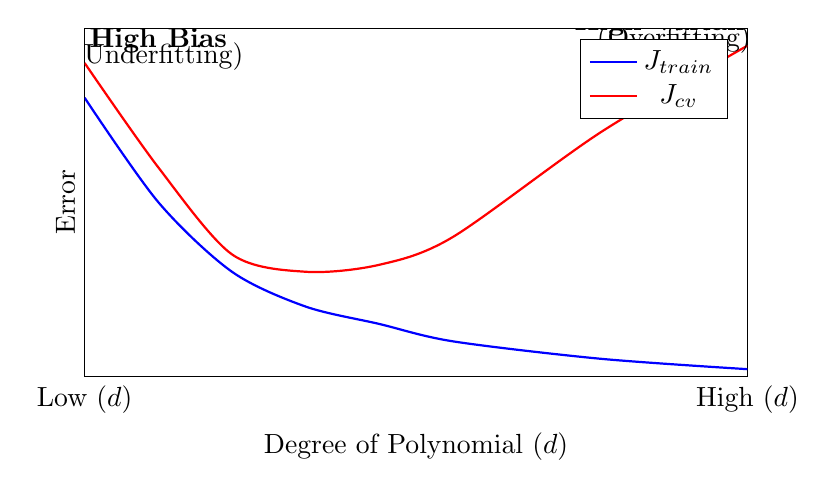
\begin{tikzpicture}
        \begin{axis}[
            width=10cm, height=6cm,
            xlabel={Degree of Polynomial ($d$)},
            ylabel={Error},
            xmin=1, xmax=10, ymin=0, ymax=10,
            xtick={1, 10}, xticklabels={Low ($d$), High ($d$)},
            ytick=\empty,
            legend pos=north east
        ]
            % J_train (Decreases as d increases)
            \addplot[blue, thick, smooth] coordinates {
                (1, 8) (2, 5) (3, 3) (4, 2) (5, 1.5) (6, 1.0) (8, 0.5) (10, 0.2)
            };
            \addlegendentry{$J_{train}$}
            
            % J_cv (Decreases then increases)
            \addplot[red, thick, smooth] coordinates {
                (1, 9) (2, 6) (3, 3.5) (4, 3) (5, 3.2) (6, 4) (8, 7) (10, 9.5)
            };
            \addlegendentry{$J_{cv}$}
            
            % Annotations
            \node[anchor=south] at (axis cs: 2, 9) {\textbf{High Bias}};
            \node[anchor=south] at (axis cs: 2, 8.5) {(Underfitting)};
            
            \node[anchor=south] at (axis cs: 9, 9.5) {\textbf{High Variance}};
            \node[anchor=south] at (axis cs: 9, 9.0) {(Overfitting)};
            
        \end{axis}
    \end{tikzpicture}
    \caption{Model Complexity vs. Error. Optimal complexity is where $J_{cv}$ is minimized.}
\end{figure}

\subsection{Learning Curves (Tanulógörbék)}
Plotting error against the number of training examples ($m$).
\begin{itemize}
    \item \textbf{High Bias:} $J_{train}$ and $J_{cv}$ converge quickly but to a high error value. Adding more data \textbf{does not} help.
    \item \textbf{High Variance:} There is a large gap between $J_{train}$ and $J_{cv}$. $J_{train}$ is low, $J_{cv}$ is high. Adding more data \textbf{likely helps}.
\end{itemize}

\section{Error Metrics for Skewed Classes (Egyenlőtlen osztályok)}
When classes are imbalanced (e.g., 99.5\% of patients are healthy), Accuracy is a misleading metric. We use Precision and Recall based on the Confusion Matrix.

\begin{figure}[H]
    \centering
    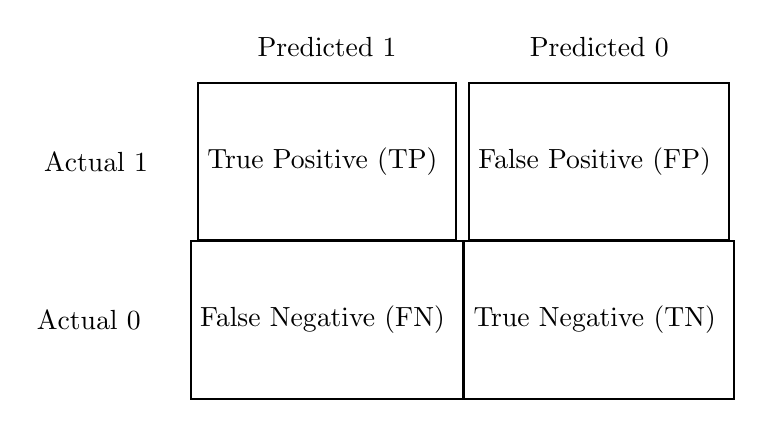
\begin{tikzpicture}
        \matrix [matrix of nodes, nodes={minimum size=2cm, align=center, draw, thick}, row sep=-\pgflinewidth, column sep=-\pgflinewidth] (cm) {
            True Positive (TP) & False Positive (FP) \\
            False Negative (FN) & True Negative (TN) \\
        };
        
        % Labels
        \node[left=0.5cm of cm-1-1] {Actual 1};
        \node[left=0.5cm of cm-2-1] {Actual 0};
        \node[above=0.2cm of cm-1-1] {Predicted 1};
        \node[above=0.2cm of cm-1-2] {Predicted 0};
    \end{tikzpicture}
    \caption{Confusion Matrix Structure.}
\end{figure}

\subsection{Metrics}
\begin{itemize}
    \item \textbf{Precision ($P$):} Of all patients we predicted as sick, what fraction actually has the disease?
    \[ P = \frac{TP}{TP + FP} \]
    \item \textbf{Recall ($R$):} Of all patients that actually have the disease, what fraction did we correctly detect?
    \[ R = \frac{TP}{TP + FN} \]
    \item \textbf{$F_1$ Score:} The harmonic mean of Precision and Recall. Used to compare models.
    \[ F_1 = 2 \cdot \frac{P \cdot R}{P + R} \]
\end{itemize}

\section{Recommender Systems (Ajánlórendszerek)}

\subsection{Problem Formulation}
Given $n_u$ users and $n_m$ items (movies), we want to predict missing ratings.
\begin{itemize}
    \item $r(i,j) = 1$ if user $j$ has rated movie $i$.
    \item $y^{(i,j)}$ is the rating given by user $j$ to movie $i$.
\end{itemize}

\subsection{Collaborative Filtering (Low Rank Matrix Factorization)}
We learn both feature vectors $\mathbf{x}^{(i)}$ for movies and parameter vectors $\boldsymbol{\theta}^{(j)}$ for users simultaneously.
\textbf{Objective Function:} Minimize squared error over all rated entries + Regularization.
\[
J(\mathbf{x}^{(1)}, \dots, \mathbf{x}^{(n_m)}, \boldsymbol{\theta}^{(1)}, \dots, \boldsymbol{\theta}^{(n_u)}) = \frac{1}{2} \sum_{(i,j):r(i,j)=1} \left( (\boldsymbol{\theta}^{(j)})^T \mathbf{x}^{(i)} - y^{(i,j)} \right)^2 + \frac{\lambda}{2} \sum_{i=1}^{n_m} \|\mathbf{x}^{(i)}\|^2 + \frac{\lambda}{2} \sum_{j=1}^{n_u} \|\boldsymbol{\theta}^{(j)}\|^2
\]
\textbf{Gradient Descent Updates:}
\begin{itemize}
    \item For movie features $x_k^{(i)}$:
    \[ x_k^{(i)} := x_k^{(i)} - \alpha \left( \sum_{j:r(i,j)=1} ((\boldsymbol{\theta}^{(j)})^T \mathbf{x}^{(i)} - y^{(i,j)}) \theta_k^{(j)} + \lambda x_k^{(i)} \right) \]
    \item For user preferences $\theta_k^{(j)}$:
    \[ \theta_k^{(j)} := \theta_k^{(j)} - \alpha \left( \sum_{i:r(i,j)=1} ((\boldsymbol{\theta}^{(j)})^T \mathbf{x}^{(i)} - y^{(i,j)}) x_k^{(i)} + \lambda \theta_k^{(j)} \right) \]
\end{itemize}

\section{Large Scale Machine Learning}
Scaling to massive datasets ($m > 10^7$) requires specialized algorithms and system architectures. We examine three variations of Gradient Descent that manage the trade-off between accuracy and computational speed.

\subsection{Batch Gradient Descent (Standard)}
In Batch Gradient Descent, we calculate the gradient of the cost function using the **entire training dataset** before making a single update to the parameters.

\textbf{Cost Function:}
\[ J_{train}(\theta) = \frac{1}{2m} \sum_{i=1}^m (h_\theta(x^{(i)}) - y^{(i)})^2 \]

\textbf{Update Rule:}
\[ \theta_j := \theta_j - \alpha \frac{1}{m} \sum_{i=1}^m (h_\theta(x^{(i)}) - y^{(i)}) x_j^{(i)} \]

\begin{itemize}
    \item \textbf{Pros:} 
    \begin{itemize}
        \item Guaranteed to converge to the global minimum for convex error surfaces (and a local minimum for non-convex surfaces).
        \item The trajectory is smooth and direct.
    \end{itemize}
    \item \textbf{Cons:} 
    \begin{itemize}
        \item Extremely slow on very large datasets because it sums over $m$ examples for every single step.
        \item Requires loading the whole dataset into memory (RAM).
        \item Cannot learn "online" (requires retraining from scratch for new data).
    \end{itemize}
\end{itemize}

\subsection{Stochastic Gradient Descent (SGD)}
Stochastic Gradient Descent approximates the gradient using a **single training example** $(x^{(i)}, y^{(i)})$ at a time. It updates the parameters immediately after looking at just one sample.

\textbf{Algorithm:}
\begin{enumerate}
    \item Randomly shuffle the dataset.
    \item Repeat for $1 \dots \text{epochs}$:
    \begin{itemize}
        \item For $i = 1 \dots m$:
        \[ \theta_j := \theta_j - \alpha (h_\theta(x^{(i)}) - y^{(i)}) x_j^{(i)} \]
    \end{itemize}
\end{enumerate}

\begin{itemize}
    \item \textbf{Pros:} 
    \begin{itemize}
        \item Much faster iterations; often converges (to a "good enough" solution) much faster than Batch GD for large $m$.
        \item Can handle datasets larger than memory.
        \item Adds noise which can help escape shallow local minima.
    \end{itemize}
    \item \textbf{Cons:} 
    \begin{itemize}
        \item The path to the minimum is "noisy" and oscillates (wanders) around the optimal value rather than settling perfectly.
        \item Loses vectorization benefits (processing 1 item is inefficient for SIMD/GPUs).
    \end{itemize}
\end{itemize}

\subsection{Mini-batch Gradient Descent}
Mini-batch GD is the standard compromise used in modern Deep Learning. It computes the gradient using a small random subset of data (a **batch**) of size $b$ (typically $b=32, 64, 128, \dots$).

\textbf{Update Rule:}
For a batch $B = \{(x^{(k)}, y^{(k)}) \mid k = i, \dots, i+b-1\}$:
\[ \theta_j := \theta_j - \alpha \frac{1}{b} \sum_{k \in B} (h_\theta(x^{(k)}) - y^{(k)}) x_j^{(k)} \]

\begin{itemize}
    \item \textbf{Advantages:}
    \begin{itemize}
        \item **Vectorization:** Modern hardware (GPUs) can parallelize the matrix operations for 64 examples almost as fast as for 1 example.
        \item **Stability:** The gradient approximation is smoother than SGD (less noise), allowing for larger learning rates.
        \item **Speed:** Much faster than Batch GD; does not require full dataset in memory.
    \end{itemize}
\end{itemize}

\begin{figure}[H]
    \centering
    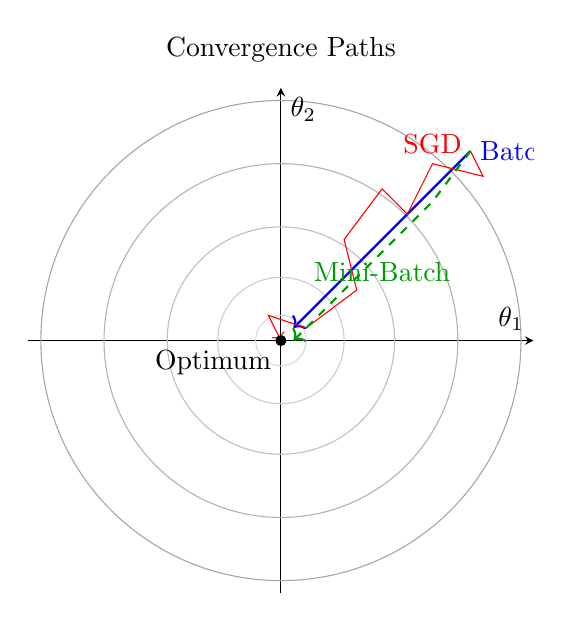
\begin{tikzpicture}
        \begin{axis}[
            width=8cm, height=8cm,
            axis lines=middle,
            xmin=-2, xmax=2, ymin=-2, ymax=2,
            xtick=\empty, ytick=\empty,
            xlabel=$\theta_1$, ylabel=$\theta_2$,
            title={Convergence Paths}
        ]
            % Contour lines
            \draw[gray!30] (0,0) circle (0.2);
            \draw[gray!40] (0,0) circle (0.5);
            \draw[gray!50] (0,0) circle (0.9);
            \draw[gray!60] (0,0) circle (1.4);
            \draw[gray!70] (0,0) circle (1.9);
            
            % Batch GD (Direct line)
            \draw[->, blue, thick] (1.5, 1.5) -- (1.0, 1.0) -- (0.5, 0.5) -- (0.1, 0.1);
            \node[blue, right] at (axis cs: 1.5, 1.5) {Batch GD};
            
            % SGD (Noisy path)
            \draw[->, red] (1.5, 1.5) -- (1.6, 1.3) -- (1.2, 1.4) -- (1.0, 1.0) -- (0.8, 1.2) -- (0.5, 0.8) -- (0.6, 0.4) -- (0.2, 0.1) -- (-0.1, 0.2) -- (0,0);
            \node[red, above] at (axis cs: 1.2, 1.4) {SGD};
            
            % Mini-batch (Smoother than SGD, not perfectly straight)
            \draw[->, green!60!black, thick, dashed] (1.5, 1.5) -- (1.2, 1.1) -- (0.8, 0.7) -- (0.4, 0.3) -- (0.1, 0.0);
            \node[green!60!black, below] at (axis cs: 0.8, 0.7) {Mini-Batch};
            
            \fill[black] (0,0) circle(2pt) node[below left] {Optimum};
        \end{axis}
    \end{tikzpicture}
    \caption{Visual comparison of convergence paths. Batch GD takes a direct path but steps are slow. SGD zig-zags significantly. Mini-batch offers a balanced path.}
\end{figure}

\subsection{Online Learning}
Used when data arrives in a continuous stream (e.g., clickstream data, search queries) and we do not store the dataset.
\begin{itemize}
    \item \textbf{Process:} Receive $(x, y) \to$ Update $\theta \to$ Discard $(x, y)$.
    \item \textbf{Adaptability:} The model can adapt to changing user preferences (concept drift) over time.
    \item \textbf{Algorithm:} Essentially Stochastic Gradient Descent (SGD) running indefinitely.
\end{itemize}

\subsection{Distributed Learning Architectures}
When data or models are too large for a single machine, we parallelize.

\subsubsection{Data Parallelism (Map-Reduce)}
The dataset is split into chunks. Each machine computes gradients for its chunk, and a central server aggregates them.
\[ \theta_{new} = \theta_{old} - \alpha \sum_{k=1}^{N_{machines}} (\text{Partial Gradient}_k) \]

\begin{figure}[H]
    \centering
    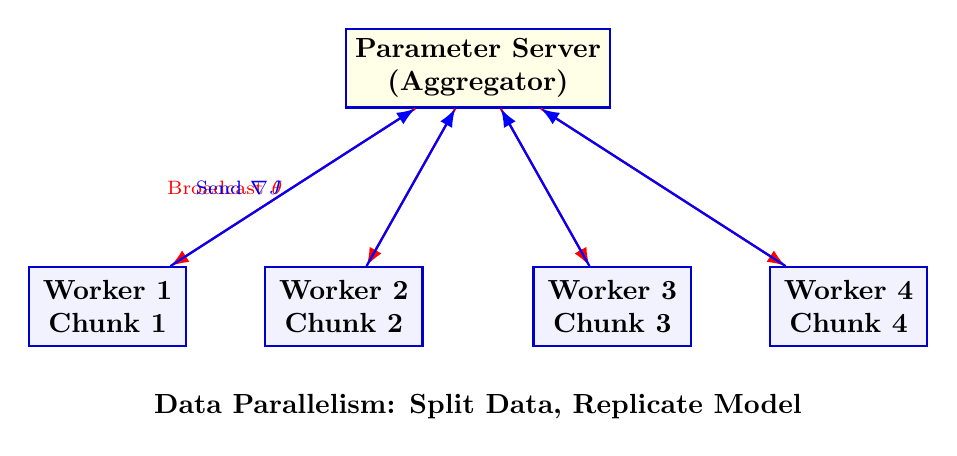
\begin{tikzpicture}[node distance=2cm]
        % Central
        \node[block, fill=yellow!10] (Master) {Parameter Server\\(Aggregator)};
        
        % Workers
        \node[block, below left=2cm and 2cm of Master] (W1) {Worker 1\\Chunk 1};
        \node[block, below left=2cm and -1cm of Master] (W2) {Worker 2\\Chunk 2};
        \node[block, below right=2cm and -1cm of Master] (W3) {Worker 3\\Chunk 3};
        \node[block, below right=2cm and 2cm of Master] (W4) {Worker 4\\Chunk 4};
        
        % Arrows
        \draw[arrow, red] (Master) -- node[left, font=\scriptsize] {Broadcast $\theta$} (W1);
        \draw[arrow, red] (Master) -- (W2);
        \draw[arrow, red] (Master) -- (W3);
        \draw[arrow, red] (Master) -- (W4);
        
        \draw[arrow, blue] (W1) -- node[left, font=\scriptsize] {Send $\nabla J$} (Master);
        \draw[arrow, blue] (W2) -- (Master);
        \draw[arrow, blue] (W3) -- (Master);
        \draw[arrow, blue] (W4) -- (Master);
        
        \node[below=3.5cm of Master, font=\bfseries] {Data Parallelism: Split Data, Replicate Model};
    \end{tikzpicture}
    \caption{Map-Reduce / Data Parallelism architecture.}
\end{figure}

\subsubsection{Model Parallelism}
Used when the \textbf{model itself} (e.g., a massive Neural Network) is too large to fit in the memory of one GPU/machine.
\begin{itemize}
    \item Different layers or different neurons of the same layer are placed on different machines.
    \item Requires high-bandwidth communication between machines to transfer activations and gradients.
\end{itemize}

\subsection{Pipeline Ceiling Analysis}
When building complex ML systems (pipelines), it is crucial to identify which component limits performance.
\begin{itemize}
    \item \textbf{Method:} Manually set the output of a specific component to "perfect" (ground truth) and measure the overall system accuracy improvement.
    \item \textbf{Goal:} Identify the "bottleneck" where engineering effort yields the highest ROI.
\end{itemize}

\begin{figure}[H]
  \tikzset{
    block/.style={rectangle, draw=blue!80!black, thick, fill=blue!5, align=center, minimum width=2.5cm, minimum height=1cm, rounded corners},
    arrow/.style={-Latex, thick},
    nodebox/.style={rectangle, draw=black, thick, fill=white, align=center},
    pipeline/.style={rectangle, draw=black, thick, fill=gray!10, align=center, minimum width=2cm, minimum height=1cm}
}
    \centering
    \begin{tikzpicture}[node distance=1.5cm]
        \node[pipeline] (Img) {Raw Image};
        \node[pipeline, right=of Img] (Text) {Text Detection};
        \node[pipeline, right=of Text] (Char) {Character Segmentation};
        \node[pipeline, right=of Char] (Recog) {Character Recognition};
        \node[right=1cm of Recog] (Acc) {Final Accuracy: 72\%};
        
        \draw[arrow] (Img) -- (Text);
        \draw[arrow] (Text) -- (Char);
        \draw[arrow] (Char) -- (Recog);
        \draw[arrow] (Recog) -- (Acc);
        
        \node[below=0.5cm of Text, font=\footnotesize, align=center] {If "Perfect":\\Acc $\to$ 89\%\\(+17\%) \textbf{High Priority}};
        \node[below=0.5cm of Char, font=\footnotesize, align=center] {If "Perfect":\\Acc $\to$ 73\%\\(+1\%) Low Priority};
    \end{tikzpicture}
    \caption{Ceiling Analysis Example (OCR Pipeline).}
\end{figure}



\end{document}